%& -job-name=presentation
\documentclass{beamer}
\usepackage{graphicx}
\usepackage{booktabs}
\usepackage[backend=biber]{biblatex}
\usepackage{color, colortbl}
\usepackage[most]{tcolorbox}
\usepackage{amsmath}
\addbibresource{sample.bib}
%Information to be included in the title page:
\title{Data Science Research Methods Assignment-3}
\usetheme{Copenhagen}
\useinnertheme{circles}
%\usecolortheme{albatross}
%\useoutertheme{Albatross}
%\usetheme[hideothersubsections]{/home/sahil/beamerports/PraterStreet}
\author{Sahil Singh}
\institute{University of Sussex}
\date{2021}

\begin{document}

\frame{\titlepage}

\begin{frame}{Introduction}

The objective of the report was to analyze a movie dataset from imdb to make reccomendations on the type of movie the studio should consider making.Our budget for production was 1.5 million.
%\begin{figure}
%	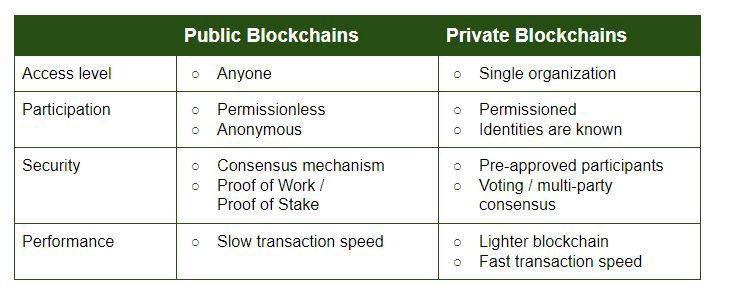
\includegraphics[width=\textwidth,height=\textheight,keepaspectratio]{privpublic.jpeg}
%	\caption{Comparision between the two types} \nocite{luxtag}
%  \label{fig:boat1}
%\end{figure}

\end{frame}
\begin{frame}{Data Analyses}
%\begin{itemize}
%\item Capital Markets
\begin{itemize}
    \item First step was to control for budget and only consider movies with a budget of less than 1.5 million.
    \item Next, a new feature, 'profit\_percentage' was calculated from the data such that,\\
    \begin{tcolorbox}[colback=red!5,colframe=green!75!black,title=]
	    $$\text{profit\_percentage}=\left(\frac{\text{gross}}{\text{budget}}-1\right)\times100$$
	    \tcblower
	    where 'gross' is just the total earning of the movie\\
	    and 'budget' is the budget of the movie

\end{tcolorbox} 

    \item We try to analyze the gross and profit of different genres through a boxplot.
	\\[1ex]
\end{itemize}

%\item Asset Management
%\begin{itemize}
%    \item Fund Launch
%    \item Fund administration
%    \item Transfer agency in asset management
%	\\[1ex]
%\end{itemize}
%\item Banking and Lending
%\begin{itemize}
%    \item Credit Prediction and Credit Scoring
%    \item Asset Collateralization
%\end{itemize}
%
%
%
%
%\end{itemize}


\end{frame}
\begin{frame}
\begin{figure}
	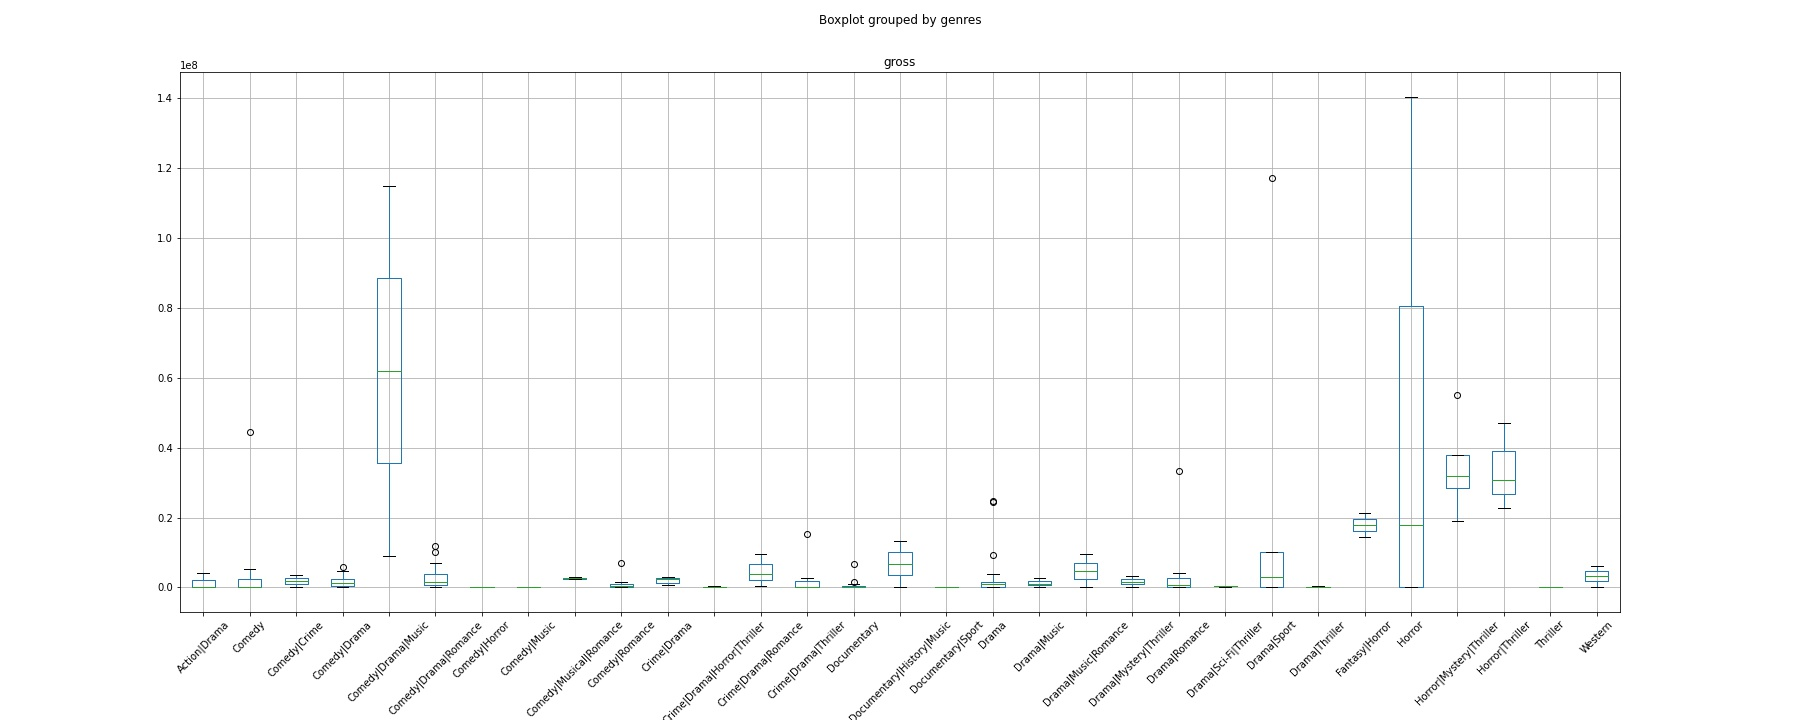
\includegraphics[width=\textwidth,height=\textheight,keepaspectratio]{test100.jpg}
	\caption{Boxplot of Gross grouped by Genres} 
	%\nocite{luxtag}
  \label{fig:boat1}
\end{figure}

\end{frame}
\begin{frame}
\begin{figure}
	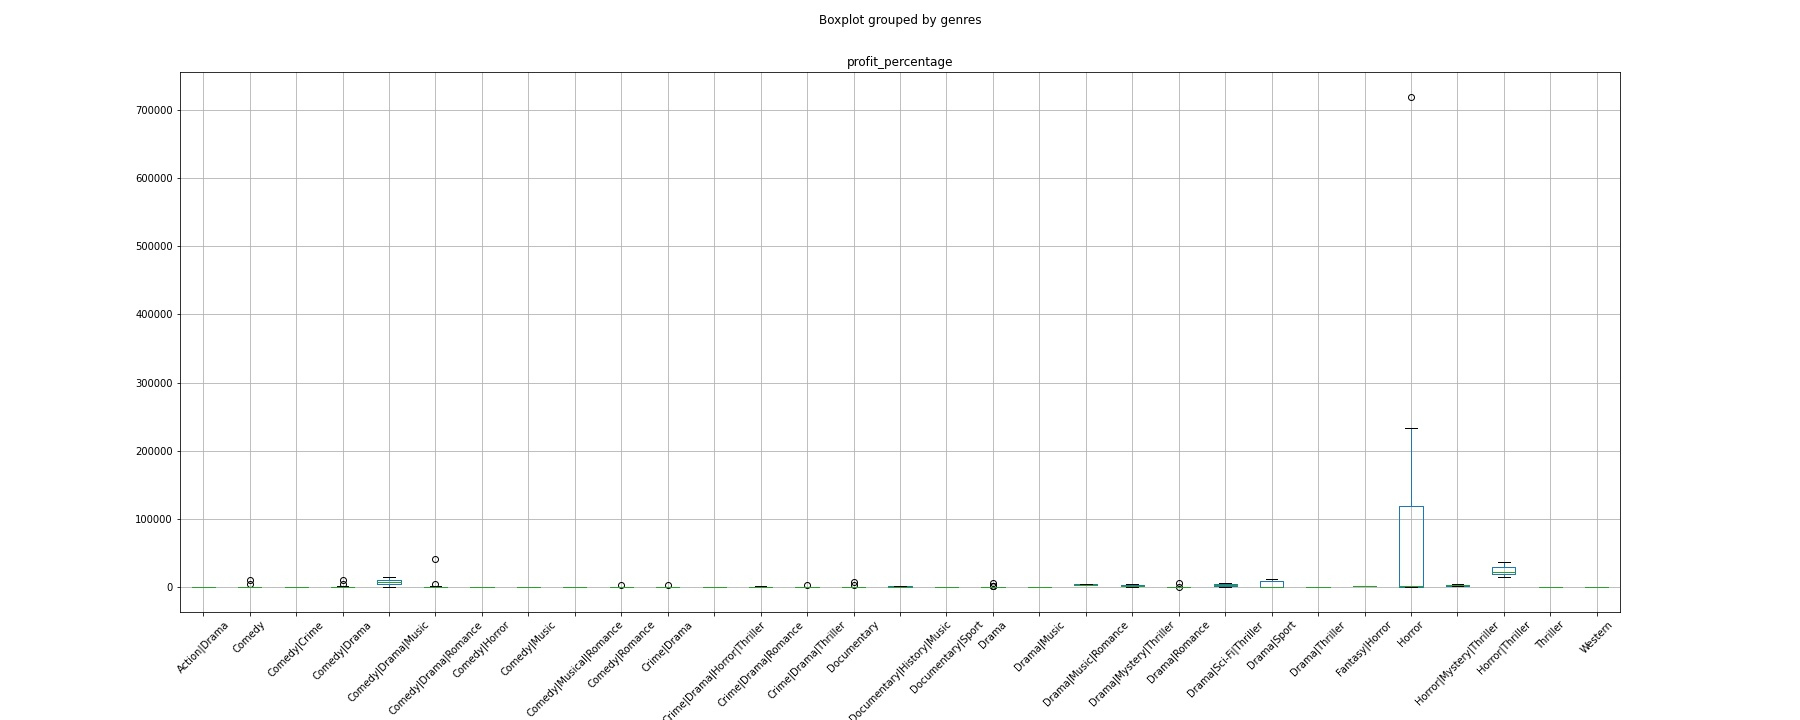
\includegraphics[width=\textwidth,height=\textheight,keepaspectratio]{test200.jpg}
	\caption{Boxplot of profit\_percentage grouped by Genres} 
	%\nocite{luxtag}
  \label{fig:boat1}
\end{figure}

\end{frame}
\begin{frame}
\begin{itemize}
\item Tried to analyze most prevelant subplots in these movies.\\
\end{itemize}

\vspace{10mm} %5mm vertical space
\centering
\begin{tabular}{lr}
\toprule
    plot\_keywords &  frequency of occurence \\
\midrule
           friend &                      16 \\
             love &                       9 \\
 independent film &                       8 \\
            drugs &                       7 \\
       friendship &                       7 \\
\bottomrule
\end{tabular}

\end{frame}

\begin{frame}{Hypothesis Generated from Data}

\begin{itemize}
\item On analysing the subplots, one sees a clear pattern that certain movie genres, for instance, Comedy/Drama/Music  have higher earnings.
\item With respect to profit\_percentage however,one sees that genres like Horror and Horror/Thriller have higher return on investment.
\item We try to test if the above mentioned genres have higher returns on average compared to other genres. 

\end{itemize}
%	\begin{itemize}
%
%\item Corda helps businesses in Banking, Capital Markets, Trade Finance, Insurance and beyond to transact directly and in strict privacy using smart contracts, reducing transaction and record-keeping costs and streamlining business operations.
%	\\[3ex]
%\item It is built for highly regulated industries.
%	\\[3ex]
%\item Delivers the core attributes of open source with enterprise functionality, services and support.
%\end{itemize}
%\end{frame}
%\begin{frame}{Challenges Faced by Corda}
%\begin{itemize}
%   \item  The absence of blocks makes the simplification of validation impossible and requires to perform complete verification of transaction history which will become more resource-consuming over time. 
%	    \\[1ex]
%    \item Corda is vulnerable to double-spending attacks which requires using special oracles to prevent attackers from performing such kind of attack.
%
%\end{itemize}
\end{frame}
\begin{frame}
\begin{tcolorbox}[colback=purple!5,colframe=blue!75!black,title=Example of a Hypothesis]
	\begin{math}
	 \mu_1  = \text{Mean of profit\_percentage of genre 'Horror'} \\
	 \mu_2  = \text{Mean of profit\_percentage of all genres \textbf{except Horror}}\\
		H_0   =  \mu_1\leq\mu_2 , \text{Null Hypothesis} \\ 
		H_1   =  \mu_1>\mu_2 , \text{Alternate Hypothesis} \\
	\end{math}
	 \tcblower
	 The above hypothesis is tested using a right-sided t-test as the 
	 sample size might be too small for a z-test.\\
	 If the p-value from the above test
	 is less than 0.05(our confidence value), we conclude that Horror movies indeed
	 earn higher than avergae compared to other genres.

\end{tcolorbox} 


%    The immutability and transparency of a Corda blockchain help empower financial institutions for gaining fast and secure access to up-to-date customer data. 
%		\nocite{alehub.io_2018},\nocite{corda}     
%\begin{itemize}
% \item Transaction finality.
% \item Ability to scale.
% \item Privacy.
% \item Legally identified parties.
% \item Developer productivity and enterprise integration.
%\end{itemize}

\end{frame}
\begin{frame}

\begin{tcolorbox}[colback=purple!5,colframe=blue!75!black,title=Bootsrapped Hypothesis Testing]

\end{tcolorbox}	
\end{frame}
\begin{frame}
\printbibliography

\end{frame}
\end{document}
